\chapter{Literature Review}
\section{terminology}
\todo[inline]{Try to avoid so many sub-subsections..terminology doesn't need to be in the own subsection...}
All definitions and terminology in this section were taken from \parencite{biggs1986graph}

\subsection{Graph Coloring and Chromatic number}
If $G$ is a graph without loops, then $G$ is $k$-colourable if we can assign one of $k$ colours
to each vertex so that adjacent vertices have different colours. If $G$ is $k$-colourable, but 
not $(k-1)$-colourable, we say that $G$ is $k$-chromatic, or that the chromatic number of $G$ is $k$, and write $\chi(G) = k$.

\subsection{Matchings}

Matching or Independent edge set in grap $G$ is subset $M$ of edges of $G$, such that no edges in $M$ share any vertice \todo{?} from $V(G)$.

Maximum matching or maximum-cardinality matching is a matching $M$ on graph $G$ that contains the largest number of edges from $G$ possible. There can exist more then one maximum matching for one graph.

Perfect matching is a matching $M$ on graph $G$ such that all endpoints of edges in $M$ form $V(G)$. $G$ can only contain perfect matching if it has even number of vertices.

\subsection{Clique and Clique number}

\subsection{Graph thickness}

Thickness $t(G)$ of a graph $G$ is the smallest number of planar graphs into which edges of $G$ can be partitioned. If there exists a union of $k$ planar graphs on one vertex set, such that the union forms graph $G$, the thickness of graph $G$ is at most $k$. Thickness of a graph $G$ is also denoted $\Theta(G)$.

\subsection{Planar Graphs}

A planar graph is a graph $G$ that can be drawn on the Euclidean plane or surface with Euler's characteristics, without any of it's edges geometrically intersecting except at the vertex. All planar graphs have thickness 1.

\subsection{Arboricity}

For an undirected graph $G$, it's arboricity, denoted as $\Upsilon(G)$, is the smallest number of edge-disjoind acyclic subgraphs whose union is graph $G$. In another words, number of forests to which edges of $G$ can be partitioned.

\subsection{Four colour Theorem}

\textcite{may1965originOf4} states that the exact origin of this problem is very vague. But one of the first appearences of this problem was in one of the lectures of A.~F.~Möbius, back in 1840. The problem remained fairly unknown until Francis Guthrie communicated it to Augustus De Morgan in around 1850.

In graph theory, subdivision of a surface on Euclidean plane, into disjoint regions formed by graph, is called a map.

The problem states that any map embedded on a plane or surface of a sphere, can be colored with only four colors, such that no adjecant regions, that share and common edge as an boundary, have the same color. In another words, for any loopless, planar graph $G$, it's chromatic number is $\chi(G) \leq 4$. \parencite{Appel1978fourColorTheorem}

Proving attempts?

\subsection{M-pire problem}

In the original four color theorem, the region is assumed to be connected. In \textcite{Heawood1947mapColourProblem} presented variation of the four color theorem, where he called a collection of $m$ disjoint regions an empire. Where empire has exactly $m$ components and it s called an $m$-pire. As in previous variation, two $m$-pires are adjecant if they share an common edge as an boundary. \parencite{jackson1985heawood}

In the graph coloring, all regions within one $m$-pire must recieve the same color.

\textcite{Heawood1947mapColourProblem} showed in 1890 that for surface $S$, where $\chi(S, M)$ is the smallest number of $k$ colors that is sufficient to color every map on surface $S$, in which m-pire has at most M disjoint regions, holds:

\begin{equation}
\chi(S, M) \leq \lfloor 1/2(6M + 1 + \sqrt[]{((6M + 1)^2 - 24E)}) \rfloor
\end{equation}

Only exceptions are for $M=1$ which is exactly the same problem as in four color theorem. He comlpetely solved the problem for $M=2$ and showed that for every $m$-pire graph with $m \geq 1$, only $6m$ colors are sufficent, setting the upper bound for this problem.
\textcite{jackson1984solution} later in 1984 solved the problem completely and showed genereal construction. 

\subsection{Earth-Moon problem}

Before Brad Jackson and Gerhard Ringel solved the $m$-pire problem, Gerhard Ringel proposed new variation of the problem where $m = 2$. With one small adjustment where the disjoint regions of said $2$-pire are in separate disjoint graphs. Making two maps, each one containing the same number of regions, the problem is as before, finding the smallest chromatic number $\chi(G)$ of disjoint union of these graphs, where region has the same colour in both graphs. 

This problem thanks to \textcite{kainen1974some} became know as Ringel’s Earth-Moon Problem. He described the two separate graphs as Earth and Moon, where countries from Earth are trying to colonize Moon.

As this is just reformulation of the $m$-pire problem, Heawood’s upper bound solution for $m = 2$ where maximum of $6m$ colors are sufficient still holds. First more suitable solution was presented in 1973 by Thom Sulanke when he found thickness-$2$ decomposition of the join of $C_5$ and $K_6$. He has presented it in correspondation between him and Martin Gardner. This graph was later presented in Scientific American in
1980. See figure below.

\begin{figure}[H]
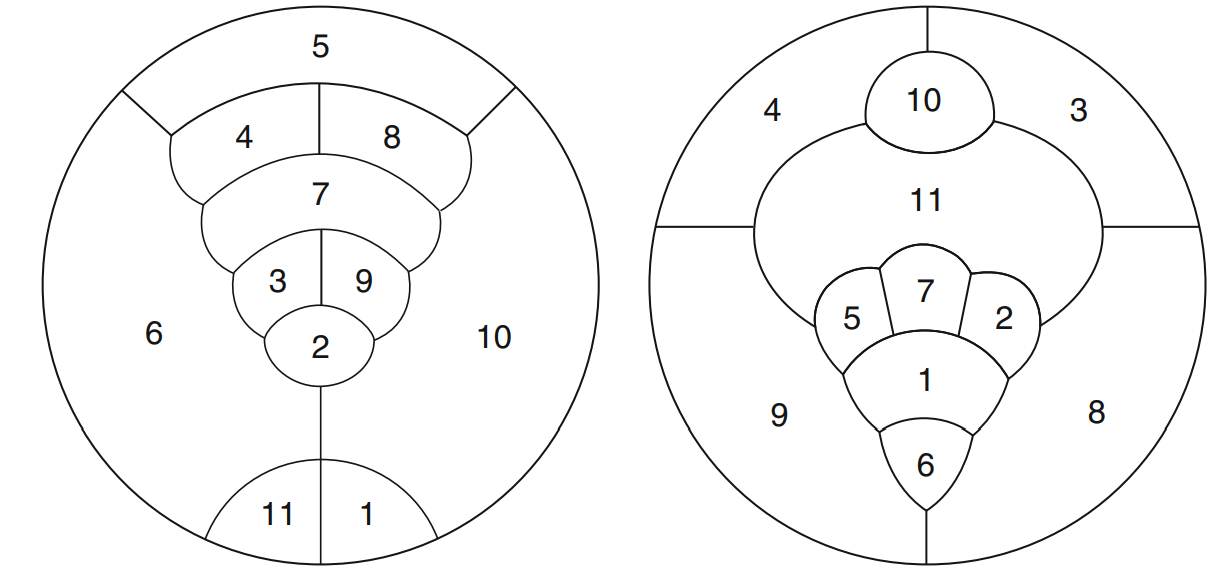
\includegraphics[width=\textwidth]{images/sulankeGraph.PNG}
\caption{Sulanke's thickness-$2$ decomposition of the join of $C_5$ and $K_6$ from Scientific American.}
\end{figure}

From later correspondece between Thom Sulanke and Gerhard Ringel, the lower bound for this problem was also set. It is know fact that $K_8$ has thickness $2$, and for every $K_n$ where $n \geq 9$ the thickness is bigger then $2$ \parencite{battle1962every}. Let $\chi_2(G)$ be a maximum chromatic number of all graphs with planar thickness $2$. For any $n$ of $K_n$ the chromatic number of any complete chraph $\chi(K_n)$ is equal to $n$, thus $\chi_2(G) \geq 8$. From this, the solution for Ringel’s Earth-Moon Problem should lie in $\{8,9,10,11,12\}$. However, Sulanke pointed out that his decomposed joined graph of $C_5$ and $K_6$ has chromatic number 9, thus $\chi_2(G) \geq 9$ and the solution lies in $\{9,10,11,12\}$.

\section{Graceful labeling}

Labeling of an graph $G$ is called graceful, if there exists an function (labeling) $f$ that from graph $G$  with $q$ edges produces injection from vertices of $G$ to set $ \{0,1, 2, \dots, q\} $ such that every edge $xy$ is assigned label $ |f(x) - f(y)| $ and all of the edge labels are distinct. Any graph that can be gracefully labeled is known as graceful graph. \parencite{Velmurugan2019graceful}

\subsection{$M$ modulo $N$ graceful labeling}
\label{graceful}

Graph $G$ is $M$ modulo $N$ labeled if there exists an function $f$ from vertex set of $G$ to set $ \{ 0, M, 
N, (N + M), 2N, (2N + M), \dots, N(q - 1), N(q - 1) + M\} $ where $f$ induces a bijection $f*$ from the edge set of G to $ \{ 0, M, N, (N + M), 2N, (2N + M),\dots, N(q - 1), N(q - 1) + M\} $, where:

\begin{equation}
f\ast (uv)=|f(x) - f(y)|\:\forall\:  v,u \in G \label{eq:gracefullBijection}
\end{equation}

\textcite{Velmurugan2019graceful} have shown and provided algorithm to construct $M$ modulo $N$ graceful labeling on every path $P_s$ for all positive integers $N$, by defining functions that recursively label edges in path $P_s$ with $s=2k$ or $s=2k+1$ length.

For $s=2k+1$, labeling each vertex $v$ in~$P$:
\begin{equation}
\begin{split}
 f(v_{2r-1}) &= N(r – 1)\: \text{\quad for $r = 1, 2, \dots, k + 1$} \\
 f(v_{2r}) &=N[2k - r] + M\: \text{\quad for $r = 1, 2,\dots, k$}
\end{split}
\end{equation}

and for $s=2k$, labeling each vertex v in P:
\begin{equation}
\begin{split}
f(v_{2r-1}) &= N(r – 1 )\: \text{\quad for $r = 1, 2,\dots, k$} \\
f(v_{2r}) &=N[2k – (r + 1 )] + M\: \text{\quad for $r = 1, 2,\dots, k$}
\end{split}
\end{equation}


\textcite{ALBERTSON20102725} has later proved using this $M$ modulo $N$ graceful labelling of Paths that every complete graph $K_{2r}$ can be partitioned into $r$ Hamiltonian paths of length $2r-1$ and all center edges of these paths form a perfect matching for said $K_{2r}$.

\section{Lexicographic product of Graphs}

Lexicographic product of two graphs $G$ and $H$, denoted $G \cdot H$ is a graph: which vertex set is cartesion product $V(G) \times V(H)$ and any two vertices $(u,v)$ and $(x,y)$ are adjecant in $G \cdot H$ if $u$ is adjecant to $v$ in $G$, $u=x$ or $v$ is adjecant to $y$ in~$H$.

This lexicographic product between any graph $G$ and complete graph $K_r$ is often called $r$-infaltion of graph $G$, denoted by $G[K_r]$ or $G[r]$.

In this inflation, every vertex v of graph $G$ is repleced by copy of $K_r$. Suppose the vertices of $G$ are labeled $v_1$,$v_2$,\dots,$v_n$, then $G[r_1, r_2,\dots,r_n]$ is the inflation of vertices of $G$ by complete graphs of sizes $ r_1$, $r_2$,\dots,$r_n$. There can exists an inflation of graph $G$, where these graphs does not have to necessarily be complete, denoting any graphs $H_1$, $H_2$, \dots, $H_n$, to replace each vertex $v_1$, $v_2$, \dots, $v_n$ of $G$, this inflation is therefore noted as $G[H_1, H_2,\dots,H_n]$ \parencite{Gethner2018toTheMoonAndBack}.

\subsection{Known properties of inflated graphs}

If the number of vertices and edges of graph $G$ are $V$ and $E$, then the number of vertices and edges of $G[r]$ are $rV$ and $\binom{r}{2} V+r2E$ respectively.

\subsubsection{Thickness}

\textcite{ALBERTSON20102725} has proven these thickness and chromatic properties of $r$-inflated graphs:
\begin{itemize}

\item If graph $T$ is a tree, then its clone is planar.
\item If $G$ has arboricity $k$,then $G[2]$ has thickness at most $k$.
\item The clone of a planar graph has thickness at most three.
\item If a graph $G$ has thickness $t$,then its clone has thickness at most $3tv$
\item The $r$-inflation of an edge maximal planar graph on  $n \geq 12$ vertices has thickness at least $r$. If the graph has more than 12 vertices, then the thickness is strictly greater than $r$.

\end{itemize}

\subsubsection{Chromatic number}

\begin{itemize}
    \item If $\chi(G) = k$  then $\chi(G[r]) = rk$
    \item If the clique number of graph $G$, $\omega(G)$, is equal to it's chromatic number $\chi(G)$ then $\chi(G[r]) = r\chi(G)$
\end{itemize}

\section{Independence ratio}
\section{Permuted layer graphs}

For planar graph $G$ with $V(H)=\{v_1,v_2,\dots,v_n\}$ vertices, let $\sigma$ be a permutation of $V(G)$. By constructing another planar graph $G'$, isomorphic to $G$ with every vertex $\sigma(v_i)$ in $G'$ labeled correspondingly to $v_i$ in $G$. After identifying $G$ and $G'$ on vertices with the same label, we then construct $H = G \cup G'$. After removing multiple edges from $H$, the resulting graph is called permuted layer graph with base $G$. If graph $H$ does not have any multiple edges, we cal $H$ a full permuted layer graph.

Permuted layer graph from base graph
\parencite{boutin2008thickness}

\section{The Hajos construction}

Let be $G_1$ and $G_2$ be two undirected graphs. One edge $(x,y) \subseteq E(G_1)$ and second edge $(u,v) \subseteq E(G_2)$. The Hajós construction constructs a new graph by combining two vertices $x$ and $u$ into one, deleting the vertices $(x,y)$ and $(u,v)$ and adding a new edge $(y,v)$.

\textcite{boutin2008thickness} have proved that for any graph $G$ the Hajos construction from graphs $H$ and $K$ satysfies $\Theta(G) = max\{\Theta(H), \Theta(K)\}$.

\section{Catlin’s graphs}

\textcite{CATLIN1979268graphs} has identified a family of inflated graphs $C_n[K_r]$, in which every vertex in $C_n$ is inflated into corresponding $K_r$. Their goal was to prove that for every $m$-chromatic graph, this graph cannot contain no subdivision of $K_n$. In their paper they have sucessfully provided an formula for chromatic number of any $C_n[K_r]$.

\section{Constructing graphs with targeted thickness}

This chapter, talks about several known methods for constructing graph with targeted thicnkess. Either by inflation or by using leyered graph construction.

\begin{enumerate}
\item \textcite{ALBERTSON20102725} proved for every $r \geq 1$, thickness for every $r$ inflated icosohedral graph $I[r]$ is equal to $r$.

They showed that for icosahedral graph $I$ and it's perfect matching $M$, every vertex in $I$, toghether with it's all neighbous, induces 5-wheel, and every edge in $M$, is an diagonal in unique quadrilateral. This allowed then to subdivide each edge in $M$ to $2r-2$ vertices and make each of the newly added vertices adjecant to the two remaining vertices of the quadliteral. Still preserving planarity. 

\begin{figure}[H]
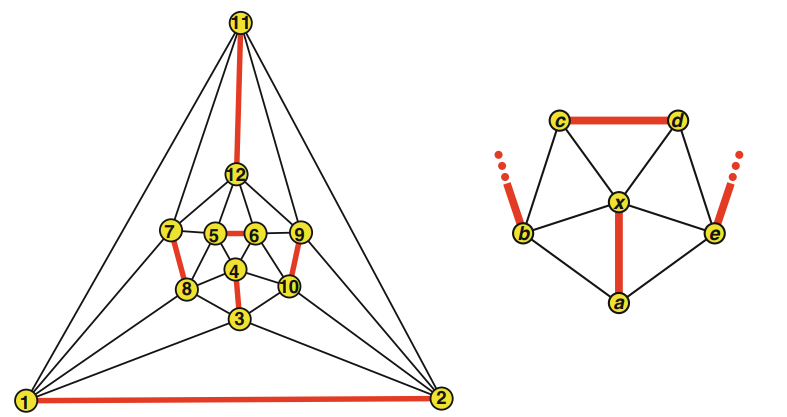
\includegraphics[width=\textwidth]{images/icosahedralMatching.PNG}
\caption{Perfect matching in $I$ and ilustrated 5-wheel\parencite{ALBERTSON20102725}.}
\end{figure}

Then by making $r$ copies of the newly modified graph, each layer called $G_1$, $G_2$,\dots,$G_r$, they proved that from each one of the former edges in $M$, thier original two vertices + the newly added $2r-2$ one's, induce path of lenght $2r$.

Using principles shown in \ref{graceful}, they proved that every edge in $I$ and it's endpoints induce $K_{2r}$ in $I[r]$ and as shown in \ref{graceful}, each one of these $K_{2r}$'s can be decomposed into Hamiltonian paths. $M$ modulo $N$ labeling can be found such that in each layer $G_1$,$G_2$,\dots,$G_r$ with subdivided edges of perfect matching, the paths fromed by the subdivisions are exactly those Hamiltonian paths in each $K_{2r}$ of $I[r]$. Union of $G_1$,$G_2$,\dots,$G_r$ represents thickness $r$ layered decomposition of $I[r]$. \parencite{ALBERTSON20102725}

\begin{figure}[H]
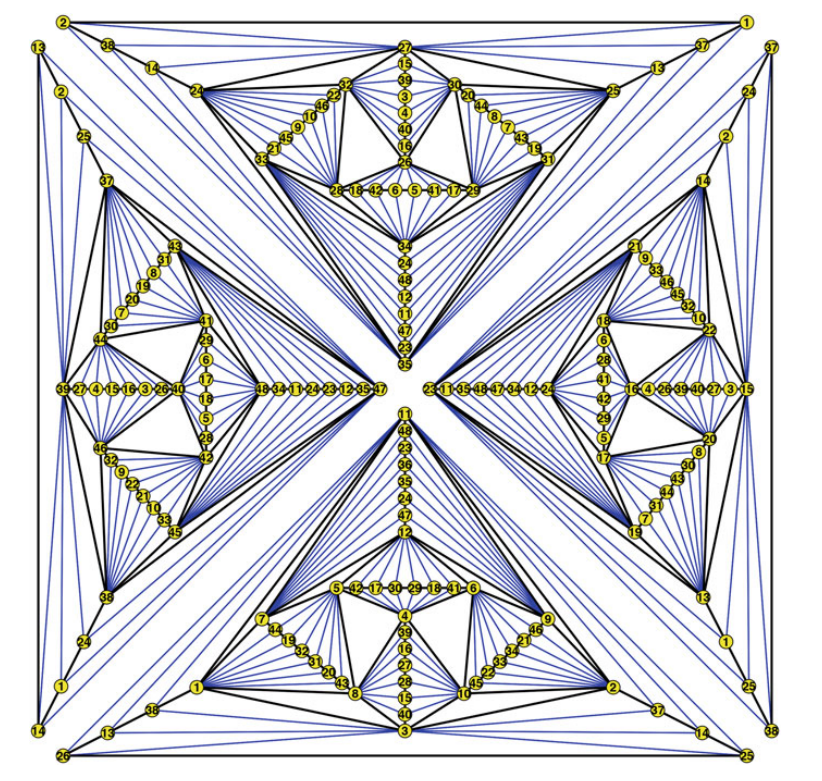
\includegraphics[width=\textwidth]{images/icosahedralDecomposition.PNG}
\caption{Planar decomposition of $I[4]$\parencite{ALBERTSON20102725}.}
\end{figure}

\item In the same paper, they provided proof for every r-inflation of a Tree graph $T$, it's thickness is at most $	\lceil r/2 	\rceil$

\item \textcite{boutin2008thickness} has presented solution for decoposing every Catlin graph $C_n[k_3]$ into 2 planar leyers for every $n \geq 4$.

For every $n \geq 4$, vertices of $C_n$ can be labeled $v_1,v_2,v_3,\dots,v_n$, all of these vertices will be expanded with $K_3$, each of these new expanded vertices labeled $\{3i - 2, 3i - 1, 3i\}$ for $ i=1,2,3,\dots,n$. Then, the $C_n[k_3]$ can be decomposed into two planar layers, first one being edge-disjoint union of three copies of paths $P_n$ of length $n$, $n$ 3-cycles, and path $P_{3n-2}$. 

First three paths being constructed from vertices: $\{1, 4, 7,\dots, 3n − 5, 3n - 2\}$, $\{n - 1, 2, 5,\dots, 3n - 7, 3n - 4\}$ and $\{3, 6,\dots, 3n-3, 3n\}$. The 3-cycles from vertices: $\{3i +1, 3i - 1 (mod3n), 3i + 3\}$ for $i = 0,1,2,\dots,n$, and the path $P_{3n-2}$ from verties: $\{3, 2, 1, 6, 5, 4,\dots, 3i, 3i - 1, 3i - 2,\dots, 3n - 3, 3n - 4, 3n - 5, 3n\}$. The 3-cycles are then embedded into first planar layer of the decomposition $G_n,1$ so they are concentric triangles. Three paths of length $n$ are then connecting the vertices of these triangles. The last path $P_{3n-2}$ is then added to add the remaining edges.

Second planar layer of the decomposition $G_n,2$ is constrcted again from edge-disjoint union of path $P_{3n-4}$ from vertices $\{ 3, 4, 8, 6, 7, 11, 9, 10,\dots,3i - 1, 3i − 3, 3i − 2,\dots, 3n - 1, 3n - 3, 3n - 2 \}$. Together with subgraph from remaining edges induced on vertices: $\{ 1,2,5,3n, 3, 3n - 2, 3n - 1,3n - 4 \}$. \parencite{boutin2008thickness}

\begin{figure}[H]
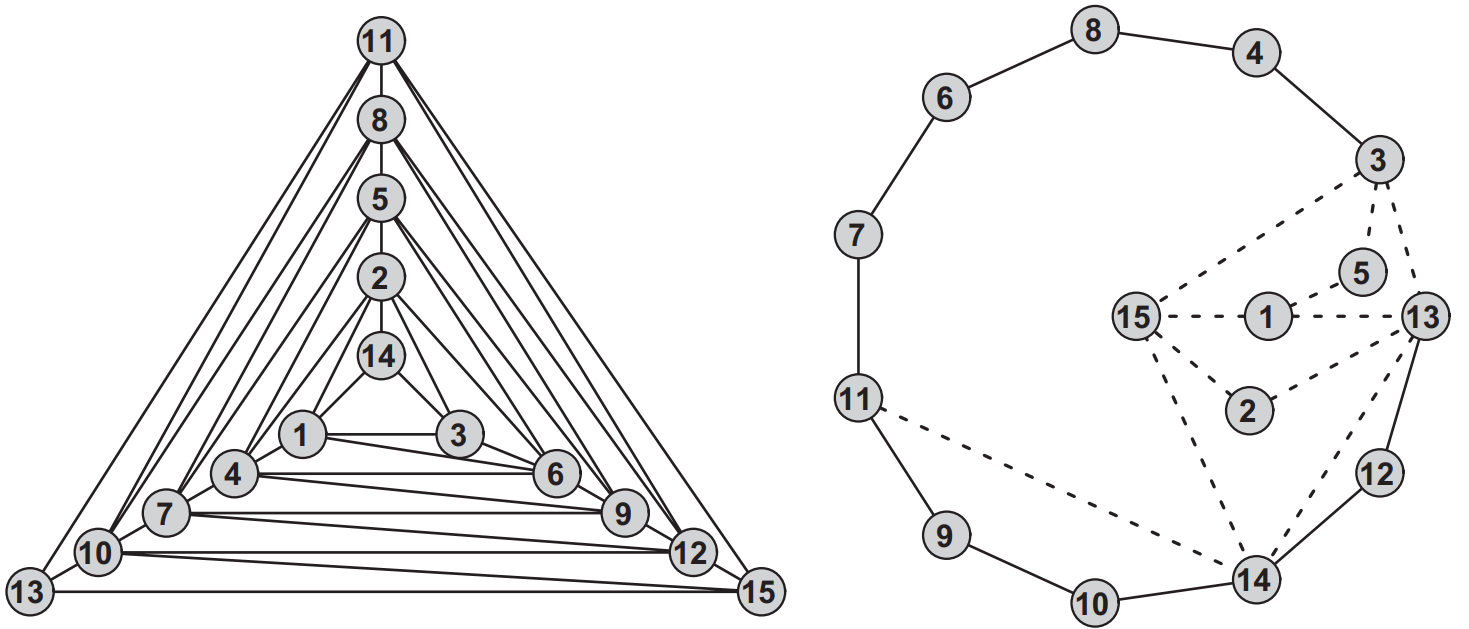
\includegraphics[width=\textwidth]{images/catlinDecomposition.PNG}
\caption{Example decomposition of $C_5[k_3]$\parencite{boutin2008thickness}.}
\end{figure}

\end{enumerate}

\section{Planar Triangulations}

\subsubsection{Surfaces?}

\subsubsection{Polyhedral Subdivision}

Let $A = a_1, a_2,\dots, a_n$ be a point set and planar graph $G$ induced by these vertices. $G$ divieds the plane into a set of regions, these regions are each bounded by a closed walk, called boundary. These regions are called $faces$. Degree of a face is the length if it's boundary closed walk. \parencite{planarGraphs2001fleck}

Definition

A subset $S$ of $\mathbb{R}^2$ is said to be $convex$ if for any two points $x$ and $y$ in $S$, line segment (edge) between $x$ and $y$ must be entirely contained in $S$.\parencite{computingCH2003smid}
 
Definition

A $convex\: hull$ of set $S$ is the smallest $convex$ set that contains $S$. It's boundary is always a convex polygon, whose vertices are points of $S$ and it's vertices are edges between those vertices. This polygon is denoted by $conv(S)$. \parencite{computingCH2003smid}

A polyhedral subdivision of set $A$ is collection $S$ of subsets $\sigma_1$,$\sigma_2$,\dots,$\sigma_n$ of $A$, called cells, such that:
\begin{equation}
\cup_{\sigma \in S} = conv(A)
\end{equation}
and: 
\begin{equation}
	\forall \sigma_1,\sigma_2 \in S, conv(\sigma_1,\sigma_2) = conv(\sigma_1) \cap conv(\sigma_2) 
	
	& \text{\ and face of \quad }\sigma_1 \cap \sigma_2 \text{\quad is also face of \quad } conv(\sigma_1), conv(\sigma_2)
\end{equation}
\subsubsection{Triangulations in planar graphs}

Polyhedral subdivision $S$ in which every said subset $\sigma_1$,$\sigma_2$,\dots, $\sigma_n$ has a face whose boundary is length 3 is called an triangulation \parencite{fisikopoulos2009triangulations}.

\subsection{Flips in planar graphs}

Flips in planar graphs are fundamental part of enumeration of different classes or types of planar graphs where certain property is met. The flip operation itself can have vast variety and generelisations of meanings. \parencite{bose2009flips}.

Once we know what specific graph class $C$ to enumerate, the flip operation $f$ needs to be precisely defined. The $flip\: graph$ is then defined as a graph, where each $n$-vertex graph of class $C$ is an vertex (object at the vertex) of the flip graph. There exists an edge between two vertices of the flip graph, if the two $n$-vertex graphs representing said vertices differ by exactly one flip operation $f$. Being said, determining how many flips $f$ is required to transform one graph of class $C$ into an another one is calculated as their distance in the flip graph \parencite{bose2009flips}.

Connectivity of the flip graph means that transforming between any of said $n$-vertex graphs in class $C$ is possible by flip operations $f$. Additionally, if the flip graph admits a Hamiltonian path or cycle, method for generating all objects in the class can be extracted \parencite{savage1997survey}.

\textcite{boutin2008thickness}, using these flip operations enumerated the class of thickness 2 graphs and planar triangulations, and genereted forty new 9-Critical graphs valid for solution of Earth-Moon problem. 

\subsubsection{Diagonal flips}

Let $r$, $s$, $t$ and $u$ be four points of set $S$. And let $T$ and $L$ be two triangulations on these vertices, with one common side, edge $us$. In the quadrilateral $rstu$, if any of the angles $rut$ and $tsr$ are less then $\pi$, dioagonal flip in these two triangles is possible. This flip operation removes the edge $us$ and inserts a new edge $rt$. Flipping the diagonal in the quadrilateral \parencite{LAWSON1972365}.

\textcite{LAWSON1972365} has proved, using diagonal flips in triangulations, for every point set $S$ and any two triangulations $T_1$ and $T_2$ on $S$, there exists a finite sequence of diagonal flips where $T_1$ can be fully transformed into $T_2$. Later, \textcite{komuro1997diagonal} has proved that this can be done in $O(n)$ time, where n is the number of vertices of $T_1$ or $T_2$.


\subsubsection{Another types of flips}

Another then diagonal flips, different types of flips were identified by \textcite{GODDARD1996121}. They have also described graph manipulation by flips more precisely.

Let $\xrightarrow[]{\mathscr{E}}$ be an symmetric and nonreflexive binary relation on graphs. Then, graph $G$ can be transformed into into another graph $H$ in $k$ steps by $\mathscr{E}$ if there exists sequence $G = G_0,G_1,G_2,\dots,G_k = H$ of transition graphs such that $G_i \xrightarrow[]{\mathscr{E}} G_{i+1}$ for $0 \leq i\: \leq k - 1$. Then the distance between said graphs $G$ and $H$ in flip graph is denoted $\delta_\mathscr{E}(G,H)$ and it is an minumim value of $k$ steps such that $G$ can be transformed into $H$.

Three new introduced edge manipulations are, edge move, edge rotation and edge slide. 
\begin{enumerate}
    \item Edge move $G_1 \xrightarrow[]{EM} G_2$ exists if there exists edge manipulation for edges $e_1 \in E(G_1)$ and $e_2 \in E(G_2)$ such that $G_2 = G_1 - e_1 + e_2$. This manipulation is denoted $\delta_{EM}$.
    
    \item Edge rotation $G_1 \xrightarrow[]{ER} G_2$ exists if there exists edge manipulation for edges  $e_1 \in E(G_1)$ and $e_2 \in E(G_2)$ such that $e_1$ and $e_2$ have one common vertex in $G_2 = G_1 - e_1 + e_2$. This manipulation is denoted $\delta_{ER}$.
    
    \item Edge slide $G_1 \xrightarrow[]{ES} G_2$  exists if there exists edge manipulation for edges $e_1 = xy \in E(G_1)$ and $e_2 = xz \in E(G_2)$ such that $y$ and $z$ are adjecant in $G_2 = G_1 - e_1 + 
    e_2$.This manipulation is denoted $\delta_{ES}$.
    
    \begin{figure}[H]
    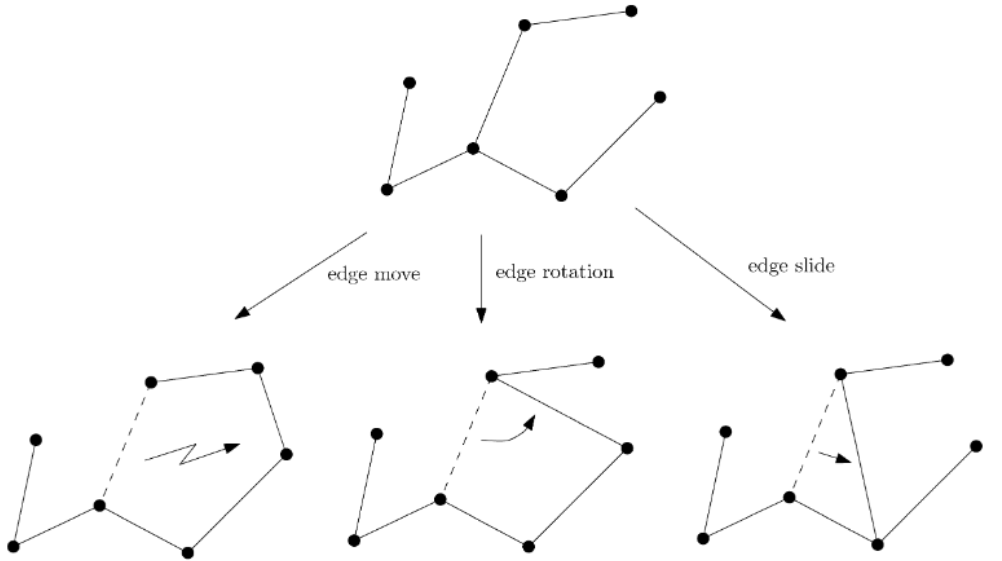
\includegraphics[width=\textwidth]{images/edgeManipulation.PNG}
    \caption{Illustration of different edge manipulations\parencite{bose2009flips}.}
    \end{figure}
    
\end{enumerate}

\subsubsection{flips and spanning trees}

\textcite{LEE1989551} also shown an interesting property in graphs under flips. If the points of an graph $G$ are in convex position, there exists a bijection between near triangulations with $n$ vertices, which are triangulations where one face does not need to be of length 3 and between binary threes with $n - 2$ internal vertices. The three from the graph $G$ can be constructed as follows: Taking one edge $e$ from $G$ and placing is as a root node of the tree, then two another edges of the triangle with edge $e$ will be drawn in into the tree as children of the root. The tree can then be constructed recursively. 

Diagonal flip in the graph $G$ can be shown in the constructed binary tree as an rotation in it. See two figures below.

\begin{figure}[H]

    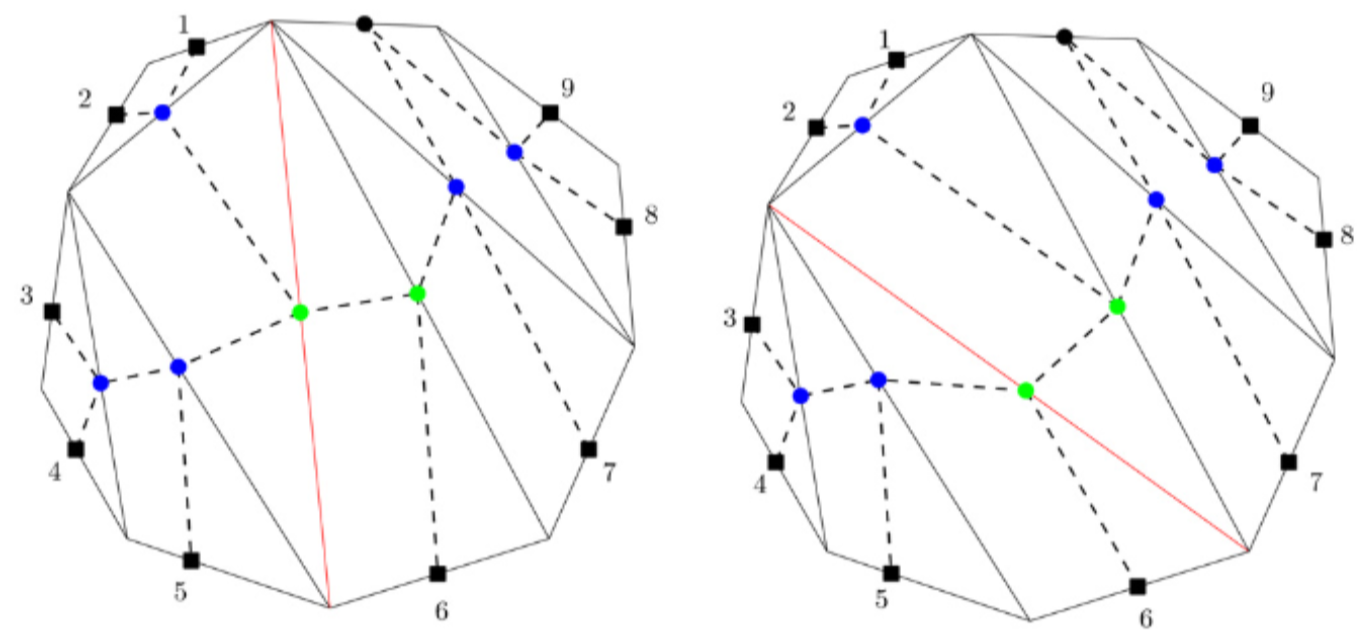
\includegraphics[width=\textwidth]{images/treeInGraph.PNG}
    \caption{Illustration of binary three in the near-triangulation.\label{fig:treeInGraph}}
\end{figure}

\begin{figure}[H]
    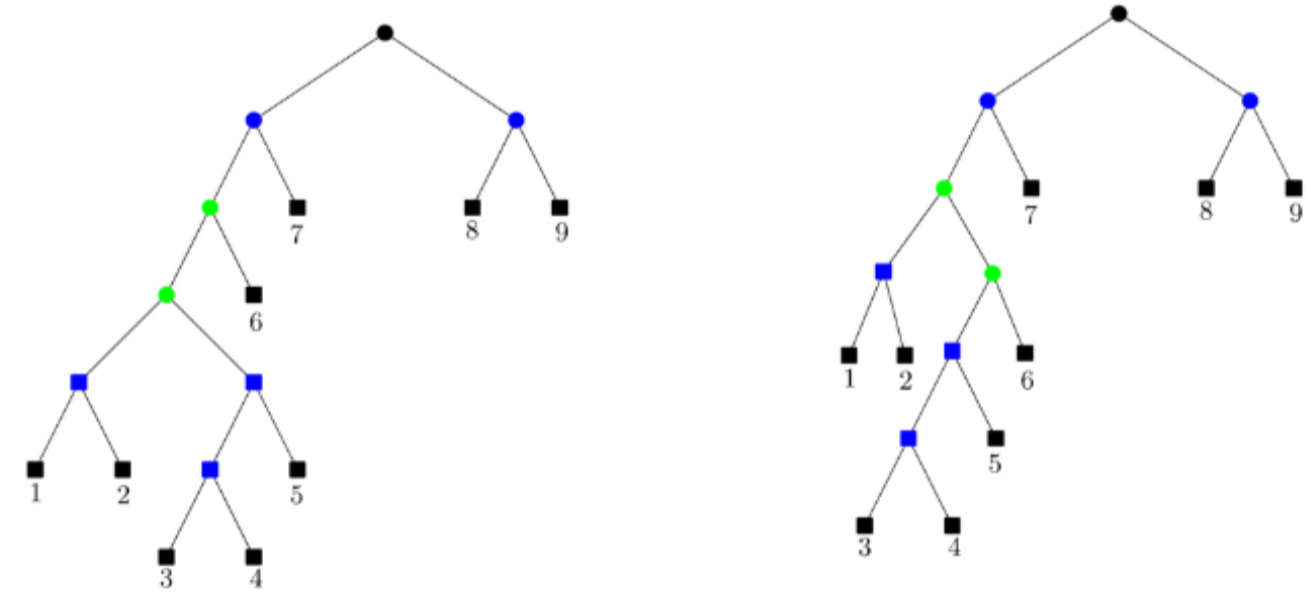
\includegraphics[width=\textwidth]{images/treeFlip.PNG} 
    \caption{Correspondence from diagonal flip in \ref{fig:treeInGraph} to rotation on the three .}
\end{figure}

\subsection{possible:}

https://core.ac.uk/download/pdf/81140248.pdf

advanced flips:

\textcite{matsumatoFlips}?

\subsection{Enumeration}

\subsubsection{Enumeration problems}

Generally, goal with enumeration problems is listing of all objects that satisfy it's conditions or properties. Enumeration problem $E$ is defined by set of instances $I$ and solution function $Sol$(I) which defines the set of solutions for given instance $I$ of the problem $E$ \parencite{schmidt2009enumeration}.

\begin{definition}
  \begin{enumerate}
    Enumeration problem $E$ is a triple $(I,Sol(),\preceq)$
    \item $I \subseteq \Sigma\ast$ is a language, previously called set of instances, where $\Sigma$ is a fixed alphabet
    \item $Sol: I \rightarrow \mathscr{P}(\Sigma\ast)$ is a function mapping set of solutions to each instance
    \item $\preceq$ is an order of solutions on $\Sigma\ast$, however I will not be dealing with orders, so $(I,Sol(),\emptyset)$ will be noted just as $(I,Sol())$
  \end{enumerate}
\end{definition}

\subsubsection{Enumeration algorithms}

Normally, efficiency is associated with polynomial running time. Models with computational power of Turing machines are all equivalent in polynomial time computability, therefore, algorithm is efficient in model A, only if it is efficient in model B. However, this cannot be applied for efficiency of enumeration problems \parencite{schmidt2009enumeration}. 

While dealing with enumeration problems, the exponential number of solutions is usually inoperative to measure in polynomial time. Enumeration algorithms are considered efficient if the total running time is polynomial in input and the output, it's complete output can be computed in polynomial time, this is called $output\ polynomial$. The notion $polynomial\ delay$ is used when the time between two successive solutions is polynomial in the input \parencite{JOHNSON1988119}.

\begin{definition}
  \begin{enumerate}
  Enumeration algorithm $A$ is for the enumeration problem $E = (I,Sol(),\preceq)$ if it satisfies following conditions:
  \item On any input $x \in I$, $A$ outputs precisely elements of $Sol(x)$, without duplicates.
  \item On any input $x \in I$, $A$ terminates in finite number of steps
  \item On any input $x \in I$, for all $u$ and $v$ in $Sol(x)$ such that $u \prec v$, $A$ outputs $u$ before $v$
  \end{enumerate}
\end{definition}

For listing all graphs, satisfying certain properties, backtracking algorithms are often used. \textcite{read1975bounds} has described and collected several backtracking algorithms and their restrictions on some of the enumeration problems in graph theory (listing cycles, paths and spanning trees in graphs).

Incremental algorithms compute targeted solution by inserting enumeration objects one by one and after each insertion, updating the solution, therefore, enumerating all possible options. Their efficiency depends essentially on the order of insertion \parencite{matousek-2001}. \textcite{edelsbrunner1987algorithms} in his book presented several algorithms to enumerate properties of graphs with these algorithms.

\textcite{fisikopoulos2009triangulations} more methods maybe 

\subsubsection{Reverse Search}

Enumeration algorithm I will be examining in detail is reverse search. This technique was originally developed by \textcite{avis1996reverse} for the purpose of generating large sets of discrete objects. First occurrence of similar method was introduced by the same authors 4 years sooner \textcite{avis1991pivoting}, however, fully introduced later in the previous paper.

Reverse search construct spanning tree, called $reverse\ search\ tree$, of a enumerated graph $G$. Nodes of this reverse search tree are precisely objects to be generated. Edges in this spanning tree are generated with $adjacency\ oracle$. The subset of edges of the reverse search tree are defined with function $f$, which is a $local\ search$ for said optimization problem defined on the set of objects that will be generated \parencite{david2000tutorial}.

"A local search algorithm on $G$ is a deterministic procedure to move from any vertex to neighboring one which is larger with respect to the objective function until there exists no better neighboring vertex." \parencite{avis1996reverse}

One vertex $v\ast$ is considered a $local\ optimal$, such vertex that does not have any neighbour larger in objective of the function. Repeated application of $f$ on every another vertex $v$ in $G$ must yield path in $G$ form $v$ to $v\ast$. The set of all these paths define the $reverse\ search\ tree$ with the root $v\ast$ \parencite{david2000tutorial}. Tracing this $reverse\ search\ tree$ from $v\ast$ is performed by tracing each it's edge(object) against its orientation, which is equal to reversing the local search algorithm. This form of backtracking is done by simply performing the search algorithm itself \parencite{avis1996reverse}. 

\begin{definition}
\subsubsection{Algorithm}

Let $G = (V,E)$ be an undirected graph with vertex set $V$ and edge set $E$. Triple $(G,S,f)$ is an $local\ search$ if $S$ is a subset of $V$ and $f$ is a function $V \setminus S \rightarrow V$ if 
\begin{enumerate}
    \item $v\ \text{and}\ f(v) \in E $ for each $v \in V \setminus S$
    \item for each $v \in V \setminus S$ there exists $k$ such that $f^k(v) \in S$
\end{enumerate}

procedural form of local search $(G,S,f)$, \parencite{avis1996reverse}:

\begin{algorithmic}

\Function{LocalSearch}{$G, S, f, v_0$}
\State $v := v_0$
\While{$v \notin S$}
    \State $v$ := $f(v)$
\EndWhile
\State output $v$
\EndFunction
\end{algorithmic}

$f$ is an $local\ search\ function$ and $G$ its $underlying\ graph\ structure$. Set $V$ is the set of candidates for solution and the set $S$ is the set of solutions. $f$ searches simply for one solution.

The trace $T$ of a local search $(G,S,f)$ is a directed graph $T = (V,E(f))$ of $G$ where

\begin{equation}
    E(f) = {(v,f(v)): v \in V \setminus S}
\end{equation}

Graph $G$ is given by $adjacency\ oracle$ if :
\begin{enumerate}
    \item Its vertices are represented by nonzero integers
    \item An integer $\delta$
    \itemis given which represents an upper bound on the maximum degree of $G$, no vertex in $G$ has bigger degree then $\delta$
    \item For $1 \leqslant k \leqslant \delta$, each vertex $v$ and number $Adj(v,k)$ returns vertex adjacent to $v$ or $0$.
    \item If there exists $k$ and $k'$ such that $Adj(v,k) = Adj(v,k') \neq 0$ for some $v \in V$, then $k = k'$
    \item The set $\{Adj(v,k): Adj(v,k) \neq 0,\ $1 \leqslant k \leqslant \delta$\}$ for $v \in V$, is exactly the set of vertices adjacent to $v$
\end{enumerate}  

Conditions 3.-5. imply that $adjacency\ oracle$ returns each vertex only once for any given $k$.

"A local search $(G,S,f)$ is said to be given by an $adjacency\ oracle$ if the underlying graph $G$ is" \parencite{avis1996reverse}.

\begin{algorithmic}
\Function{ReverseSearch}{$Adj(), \delta, S, f()$}

\For{\texttt{each vertex $s \in S$}}
    \State $v := s$;
    \State $j := 0$;
    \Repeat
        \While{$k < \delta$}
            \State $j := j + 1$;
            \State $next := Adj(v, j)$;
            \If{$next \neq 0$}
                \If{$f(next) = v$}
                    \state $v := next$;
                    \state $j := 0$;
                \EndIf
            \EndIf 
        \EndWhile
        \If{$v \neq s$}
            \state $u := v$;
            \state $v := f(v)$;
            \state $j := 0$;
            \Repeat
                \state $j := j + 1$
            \Until{$Adj(v, j) = u$}
        \EndIf
    \Until{$v =s$ and $h = \delta$}
\EndFor

\EndFunction
\end{algorithmic}

\end{definition}


\section{Programming language selection}

This section will go thought comparison between using C language, another imperative languages and functional programming language, more specifically Haskell, for graph theory focused algorithms or problems.

C

Conventional programming languages, like C, are stateful. Most of the advantages for using these programming languages for graph theory comes from being able to access the state. Some algorithms inherently require this access for reduction of their complexity.

In imperative programming languages, the data structures needed for efficient implementation of some the algorithms require explicit shared access to them. Where local actions in this data structure makes a global change to it. 

Often, different approaches for problems or solution for algorithms require different representation for graphs in these languages \parencite{king1996functional}. We can see this in chapter below, when comparing multiple C libraries which provide this representation, each one differently.

Haskell

In this paradigm most usually the programs or sub parts of these programs (functions) are designed as sequences of transformations on the input data. The program of the algorithm itself is composed together from smaller,simpler routines (functions), where the main focus is what the intermediate data between these routines should be \parencite{king1996functional}.

\textcite{king1996functional} States several advantages from functional paradigm for graph theory programming.

The ability to decompose the algorithm into smaller routines greatly contribute to provability of the problems. Pure functional solutions are referentially transparent, which means every expression can be replaced with its corresponding value without changing the behaviour of the program, also contributing to verifying programs correctness. 

The data flow between smaller routines can be more easily truncated and optimized by making these exchanges of data smaller, essentially reducing steps. 

Again, these smaller routines can be more easily reused in the code, more easily then in imperial languages as in functional languages the emphasis on data types is not so prevalent, meaning manipulation of data with different types is much easier.

He also describes on few algorithms and examples where in functional programming, memory management is not an issue as in typical imperative language.

HS vc C vs Java

\textcite{fender_2011} Has provided quick comparison for few algorithm in Haskell, Java and C++ for k-coloring of an undirected graph where $k=3$. Graphs for algorithm speeds comparison can be seen below.
 
\begin{figure}[H]
    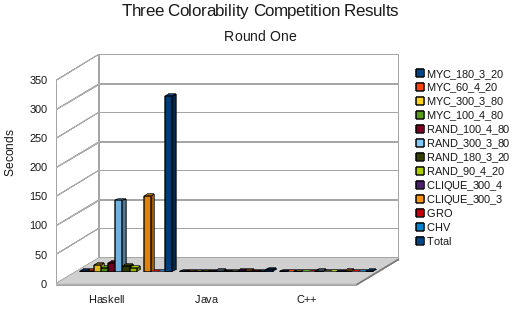
\includegraphics[width=\textwidth]{images/comparison3langs.png}
    \caption{Comparison between run speeds for 3-coloring problem for Haskell, Java and C++ \parencite{fender_2011}}
\end{figure}
\begin{figure}[H]
    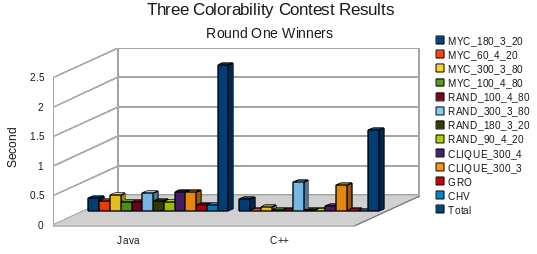
\includegraphics[width=\textwidth]{images/comparison2langs.png}
    \caption{Comparison between run speeds for 3-coloring problem for only Java and C++ \parencite{fender_2011}}
\end{figure}

Different Graph specific languages:

Multiple programming languages specialized for graph theory have been made. GRAMAS, \textcite{pape1979gramas} is such language which is very similar to Algol. GEL (Graph Exploration language), \textcite{erwig1992graph} is a functional language which provides many graph exploration operators, use-full in graph algorithms \parencite{king1996functional}. 

Mathematica, \textcite{wolfram1991mathematica} is an very important programming language/environment for discrete mathematics. It provides incredible amount of mathematical tools. However, for most of graph theory algorithms, it is inefficient and its time complexity becomes a drawback for larger graphs \parencite{king1996functional}. 

Complexity comparison:

At the end of his paper, \textcite{king1996functional} stated that for different algorithms and different data, the comparison factor between C and Haskell will always be different. However, e has shown the magnitude of speed difference between Haskell and C language for biconnected components algorithm by \textcite{tarjan1973efficient} for few graph sizes and latest implementation of this algorithm in GraphBase \parencite{knuth1993stanford}. This comparison can be seen in table below.

\begin{figure}[H]
    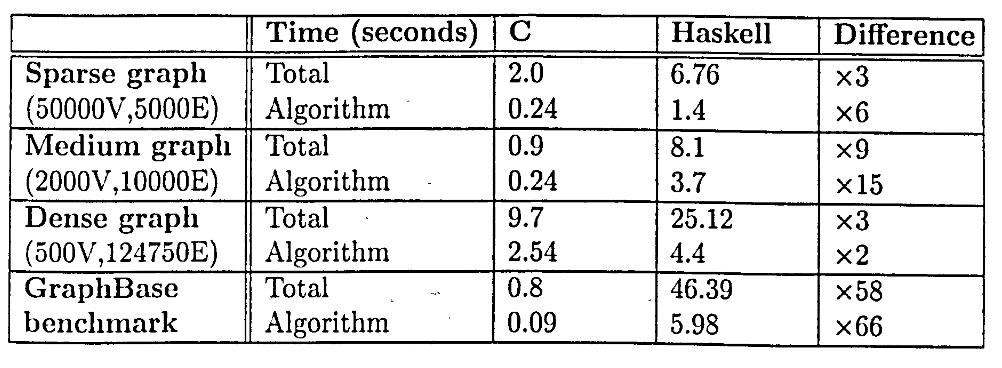
\includegraphics[width=\textwidth]{images/haskelVsC.png}
    \caption{biconnected components algorithm speeds for C and Haskell \parencite{king1996functional}}
\end{figure}

\subsection{Libraries}

The most efficient way of achieving the best asymptotic complexities is through several basic routines to manipulate the graph data structures. Re implementing these data structures and routines would be a problem on it's own so the obvious approach is to have library of these highly tuned routines. 

Two of the most notable libraries are LEDA from \textcite{mehlhorn1989leda} and Stanford GraphBase from  \textcite{knuth1993stanford}. Both of these libraries are implemented imperatively, LEDA in C++ and GraphBase in C language. Both of them provide excellent functionality while still being efficient even in memory management. For my further work, i will not be using C++ so GraphBase will be my main choice for library. It is freely available and can be downloaded from stanfords ftp server (ftp.cs.stanford.edu). \textcite{king1996functional} states that GraphBases does not provide complete set of routines for ever\ graph problem, however, it does provide necessary routines for my work and will be more then enough. Its style of presentation is also highly sophisticated. Graphbase is compatible with Knuth's CWEB, which is system of structured documentation that can be translated to C and/or TEX.


Another notable graph library in C is CGraph from \textcite{cesar-2013}, which was developed primapy for complex networks research. It also provides great amount of routines and excellent memory management of graph data structures. This is my backup choice in case GraphBase would not be sufficient. 

The Boost Graph Library (BGL) from \textcite{siek2002boost} is C++ library, however, additionally provides great support for parallelism and its generic interface provides high level abstraction and this library therefore has smaller learning  curve. 

As functional paradigm was mentioned in previous chapters, Haskell provides and maintains a graph library, developed by University of Glasgow in 2002. Data.Graph, which adds graph data structure and routines associated with it to Haskell \parencite{UniOfGlasgow2002}.

\subsubsection{CWEB}

\section{Current software solutions}

nauty

geng


